\documentclass{article}

\usepackage[utf8]{inputenc}
\usepackage[backend=biber, style=ieee]{biblatex}
\usepackage[a4paper, total={170mm,257mm}, left=20mm, top=20mm]{geometry}
\usepackage{graphicx}
\usepackage{titling}
\usepackage{amsfonts}
\usepackage{amsmath}
\usepackage{lmodern}
\usepackage{physics}
\usepackage{tikz}
\usepackage{booktabs}
\usepackage{pgfplots}
\usepackage{fancyvrb}
\usepackage{pmboxdraw}
\usepackage{fancyhdr}
\usepackage{parskip}
\usepackage{float}

\setlength\parindent{0pt}
\pgfplotsset{compat=1.18}
\usetikzlibrary{calc}
\setlength{\headheight}{5mm}

\addbibresource{citations.bib} % Imports bibliography file
 
\fancypagestyle{plain}{%  the preset of fancyhdr 
  \fancyhf{} % clear all header and footer fields
  \fancyhead[L]{UML Project Proposal}
  \fancyhead[R]{\theauthor}
}

\makeatletter
\def\@maketitle{%
  \newpage
  \null
  \vskip 1em%
  \begin{center}%
  \let \footnote \thanks
    {\LARGE \@title \par}%
    \vskip 1em%
    {\@author}%
  \end{center}%
  \par
  \vskip 1em}
\makeatother

\title{\textsc{Forg}: File Organization by Embedding Files According to File Tree Distance}
\author{Alex Chen, Geoffrey Wu, Gilbert Yang}

\begin{document}

\maketitle

\section{Introduction}

Modern file systems contain a wealth of data in terms of files and their ``semantic'' similarity. If we view a file system as a tree with files as leaf nodes, then the tree distance between leaf nodes A and B is a good measure of similarity between files A and B. For example, \texttt{log1.txt} and \texttt{log2.txt} could appear in the same parent \texttt{logs/} directory.

One could learn an embedding function $f$ that maps files to a metric space that best matches the tree metric. This includes hyperbolic spaces, as it has been shown that they can effectively embed tree-based data \cite{sarkar2011low} \cite{sala2018representation}. Once we compute such an embedding function, given a set of new files, we can embed each using $f$ and run hierarchical clustering \cite{murtagh2012algorithms} to “generate” a reasonable file tree.

Such a model can be trained on different example repositories to produce models that perform well in different contexts. For example, training on GitHub repositories will produce a model that organizes files in a way that is useful for software projects. Meanwhile, training on, say, the filesystem of an operating system will produce a model that is better adapted to organizing non-text (binary) files. The latter case may be particularly useful for organizing a user's internet downloads.

The code for our method can be found on GitHub: \url{https://github.com/forggers/forg}.

\subsection{Related Work}

Previous work has shown that embedding into hyperbolic spaces is effective at preserving the tree-distance metric \cite{sarkar2011low} \cite{sala2018representation}.

Similar work has been done in \cite{verma2012learning}, which learns similarity metrics using the class taxonomy of multi-class data. However, the goal there is to ``determine the correct placement of a new category that was not part of the original taxonomy, and can provide effective classification amongst categories local to specific subtrees of the taxonomy.'' Although Verma's work also explores learning a tree structure of some sort, the ultimate purpose and applications of the two papers are distinct.

Embeddings of semantic content of individual files have been done before, such as in the context of retrieval-augmentation-generation (RAG) systems that are common in Large Language Models (LLMs) \cite{caspari2024beyond}. These embeddings have also been used for organizing files: such as k-means clustering for big data and search \cite{laxmi2020charismatic}, file organization through file labeling \cite{abbas2023automated}, and even combining the two approaches to cluster and label files to sort them into folders \cite{raza2022content}.

However, unlike the previous approaches outlined, our approach is the first embedding and hierarchical clustering procedure that trains on the tree metric over the file directory and can directly create a new file directory structure, without going through an intermediate labeling step.

\section{Background}

We present a brief overview of concepts that are used in our project.

\subsection{Metric Spaces and Embeddings}

A metric space $(X, \rho)$ is a set $X$ equipped with a distance function $\rho: X \times X \rightarrow \mathbb{R}$, which gives the distance between pairs of elements. $\rho$ must satisfy the following four properties for all $x,y,z \in X$: 1) Non-negativity: $\rho(x,y) \geq 0$; 2) Positivity: $\rho(x,y) = 0 \iff x = y$; 3) Symmetry: $\rho(x,y) = \rho(y,x)$; 4) Triangle inequality: $\rho(x,y) \leq \rho(x,z) + \rho(z,y)$.

\subsubsection{Trees as Metric Spaces}

Consider a set $X$ where elements are nodes in a tree. In this project, we assume all edge weights in a tree equal 1. A valid distance function $\rho$ can be defined as the length of the shortest path between two nodes. This satisfies the properties of a metric space.

\begin{figure}[H]
  \centering
  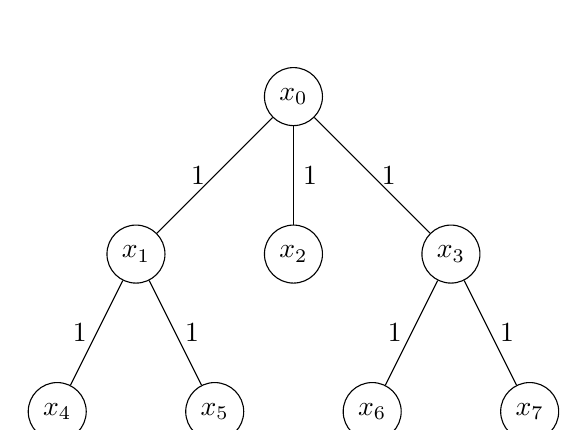
\begin{tikzpicture}
    % Nodes
    \node[circle, draw] (A) at (0,0) {$x_0$};
    \node[circle, draw] (B) at (-2,-2) {$x_1$};
    \node[circle, draw] (C) at (0,-2) {$x_2$};
    \node[circle, draw] (D) at (2,-2) {$x_3$};
    \node[circle, draw] (E) at (-3,-4) {$x_4$};
    \node[circle, draw] (F) at (-1,-4) {$x_5$};
    \node[circle, draw] (G) at (1,-4) {$x_6$};
    \node[circle, draw] (H) at (3,-4) {$x_7$};

    % Edges with distances
    \draw (A) -- node[midway, fill=none, left] {$1$} (B);
    \draw (A) -- node[midway, fill=none, right] {$1$} (C);
    \draw (A) -- node[midway, fill=none, right] {$1$} (D);
    \draw (B) -- node[midway, fill=none, left] {$1$} (E);
    \draw (B) -- node[midway, fill=none, right] {$1$} (F);
    \draw (D) -- node[midway, fill=none, left] {$1$} (G);
    \draw (D) -- node[midway, fill=none, right] {$1$} (H);
  \end{tikzpicture}
  \caption{An illustration of a tree metric space. As an example, the distance between $x_2$ and $x_4$ is $3$.}
  \label{fig:tree-metric-space}
\end{figure}

\subsubsection{Distance-Preserving Embeddings}

Given elements of a metric space, we are often interested in embedding them into a lower-dimensional space in a way that preserves distances. Formally, an embedding is a mapping $f: X \rightarrow Y$, from metric space $(\rho, X)$ to metric space $(\sigma, Y)$. To preserve distances means to find an $f$ such that for all $x,y \in X$, $\sigma(f(x),f(y)) \approx \rho(x,y)$. Later, we will discuss ways of quantifying the quality of an embedding.

\subsection{Hierarchical Clustering}

A clustering of a dataset into $k \in \mathbb{N}$ clusters is a partition of the dataset into $k$ sets, where points in a set are ``similar'' for some measure of similarity. Hierarchical clustering builds nested clusters by merging or splitting them successively. These nested clusters can be visualized in a tree-like format in a dendrogram. Agglomerative clustering is the bottom-up approach of hierarchical clustering that merges together clusters. The branch lengths in the computed tree correspond to the ``distance'' between two clusters, and at each step, the two clusters with the smallest distance between them are merged together. By varying the distance function between two clusters, we obtain different kinds of agglomerative clustering: \cite{murtagh2012algorithms} \cite{müllner2011modernhierarchicalagglomerativeclustering}

\begin{itemize}
  \item Single-linkage: between two clusters $X, Y$, the distance function is the minimum of $d(x, y)$ over all $x \in X$ and $y \in Y$.
  \item Complete-linkage: between two clusters $X, Y$, the distance function is the maximum of $d(x, y)$ over all $x \in X$ and $y \in Y$.
  \item Ward clustering: between two clusters $X, Y$, the distance function is the sum of the squared distances between all points in $X$ and all points in $Y$. Intuitively, this minimizes within-cluster variance.
\end{itemize}

\subsection{Large Language Models and Tokenizers}

Large language models (LLMs) are trained on vast amounts of internet text to learn the distribution over candidate tokens given a sequence of input tokens. An LLM's vocabulary is a set of tokens; each token is a string of characters. A common pre-processing step is to convert input text into a sequence of tokens via a \emph{tokenizer}.

Ultimately, an LLM ``sees'' tokens, so the choice of vocabulary is crucial. One common way to choose tokens is to consider a sample body of text and choose the top $V$ most frequently occurring $n$-grams (over all $n\ge 1$). This results in many tokens being parts of words, which can be useful for capturing the structure of natural language.

Most LLMs today use the transformer architecture, which uses self-attention mechanisms to model dependencies between tokens. First, the model learns token embeddings. In addition, the model learns projection matrices that map tokens into a latent space that better captures similarity structures. Each layer of the transformer uses this mechanism to allow tokens to ``pay attention'' to other tokens. As the input is passed through the layers, the model refines the meaning of each token in the context of the entire input.

After being trained on the internet, the model learns an internal representation of language that allows it to best complete input text. Ultimately, the distribution of candidate tokens output by an LLM is a function of the final hidden state of the model (i.e., the refined token embeddings at the last layer). Therefore, this final hidden state contains an abstract representation of the input text---suitable for downstream NLP tasks.

\section{Hyperbolic Geometry}

Hyperbolic geometry is a non-Euclidean geometry characterized by a constant negative curvature. Hyperbolic spaces are natural candidates for embedding trees \cite{sarkar2011low} \cite{sala2018representation}. Many models of hyperbolic space exist, including the hyperboloid, Poincaré disk, Poincaré half-plane, and Klein disk models. We will focus on the Poincaré disk model because it is easy to visualize.

\subsection{Poincaré Disk Model}

The Poincaré disk model of hyperbolic space maps points in the hyperbolic plane to points in the unit disk (in Euclidean space). The distance between two points with coordinates $\mathbf x_1$ and $\mathbf x_2$ in the \emph{ambient} Euclidean space is
\begin{align}
  d(\mathbf x_1, \mathbf x_2)
  = \text{arcosh} \qty[1 + 2 \frac{\norm{\mathbf x_1 - \mathbf x_2}^2}{\qty(1 - \norm{\mathbf x_1}^2) \qty(1 - \norm{\mathbf x_2}^2)}] \; . \label{eq:poincare-distance}
\end{align}

Geodesics are defined as the shortest paths between two points. In the Poincaré disk model, geodesics are arcs of circles that intersect the boundary of the disk at right angles. For any two points in the Poincaré disk, there is a unique geodesic connecting them.

\begin{figure}[H]
  \centering
  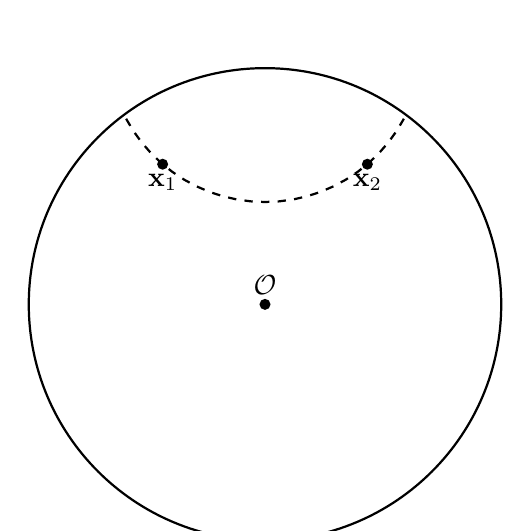
\begin{tikzpicture}
    % Draw the unit circle (Poincaré disk boundary)
    \draw[thick] (0,0) circle (3);
    % Draw the geodesic arc
    \draw[dashed, thick] plot[domain=-1.08:1.08] ({2*sin(\x r)},{-2*cos(\x r) + 3.3});
    % Draw points
    \fill (0,0) circle (0.07) node[above] {$\mathcal O$};
    \fill (-1.3,1.78) circle (0.07) node[below] {$\mathbf x_1$};
    \fill (1.3,1.78) circle (0.07) node[below] {$\mathbf x_2$};
  \end{tikzpicture}
  \caption{Poincaré disk with a geodesic between two points.}
  \label{fig:poincare-disk}
\end{figure}

\subsection{Normalizing $\mathbb{R}^D$ Output into the Poincaré Disk}

The embedding function $f$ that we use is a multi-layer perceptron that outputs vectors in $\mathbb R^D$. When using hyperbolic spaces, the Poincaré disk model requires the output to be in $\mathcal H^D$. Namely, the output must be in the unit ball $\qty{\mathbf y \in \mathbb R^D : \norm{\mathbf y} < 1}$. This requires us to use some normalization technique.

The simplest strategy is to clip the output norms to $1-\epsilon$, where $\epsilon$ is sufficiently large to avoid numeric issues that arise when computing distances near the edge of the Poincaré disk. This strategy is problematic in practice because embedded points get ``stuck'' at the boundary of the disk, due to embedding gradients being zero in the radial direction after clipping.

\begin{figure}[H]
  \centering
  \begin{tikzpicture}
    % Draw the unit circle (Poincaré disk boundary)
    \draw[thick] (0,0) circle (3);
    % Draw the smaller dotted circle (1 - epsilon)
    \draw[thick, dotted] (0,0) circle (2.7);
    % Draw radial lines from the origin to the points (going past the boundary)
    \draw[dotted] (0,0) -- (4, 0);
    \draw[dotted] (0,0) -- (-4, 0);
    \draw[dotted] (0,0) -- (0, 4);
    \draw[dotted] (0,0) -- (0, -4);
    \draw[dotted] (0,0) -- (2.83, 2.83);
    \draw[dotted] (0,0) -- (-2.83, -2.83);
    % Place points on the smaller circle
    \fill (2.7, 0) circle (0.05);
    \fill (-2.7, 0) circle (0.05);
    \fill (0, 2.7) circle (0.05);
    \fill (0, -2.7) circle (0.05);
    \fill (1.91, 1.91) circle (0.05);
    \fill (-1.91, -1.91) circle (0.05);
    % Draw original points outside the disk (fill + outline)
    \fill[white] (3.5, 0) circle (0.05);
    \draw[gray]  (3.5, 0) circle (0.05);
    \fill[white] (-3.3, 0) circle (0.05);
    \draw[gray]  (-3.3, 0) circle (0.05);
    \fill[white] (0, 3.8) circle (0.05);
    \draw[gray]  (0, 3.8) circle (0.05);
    \fill[white] (0, -3.7) circle (0.05);
    \draw[gray]  (0, -3.7) circle (0.05);
    \fill[white] (2.5, 2.5) circle (0.05);
    \draw[gray]  (2.5, 2.5) circle (0.05);
    \fill[white] (-2.7, -2.7) circle (0.05);
    \draw[gray]  (-2.7, -2.7) circle (0.05);
  \end{tikzpicture}
  \caption{Poincaré disk with embedded points clipped to radius $1 - \epsilon$.}
  \label{fig:poincare-disk-epsilon}
\end{figure}

Ideally, we want points to get arbitrarily close to the boundary of the Poincaré disk. This is because there is more \emph{space} to fit tree-like structures near the boundary. Furthermore, we want a strategy that reserves ``more bits'' of floating point precision for regions near the boundary. One such strategy is to apply a nonlinear transformation $g: \mathbb R^+ \to [0, 1)$ to the norms of MLP-outputted vectors. $g(r) = \tanh(r)$ is a possible candidate, as $\dv{g}{r}$ diminishes for small $r$. In other words, a large share of the domain $r \in \mathbb R^+$ is mapped to the region near $1$ in $[0, 1)$.

We instead choose to use a very similar transformation:
\begin{align}
  g(r) = \sqrt{1 - e^{-r^2}} \; . \label{eq:radial-transformation}
\end{align}

\begin{figure}[H]
  \centering
  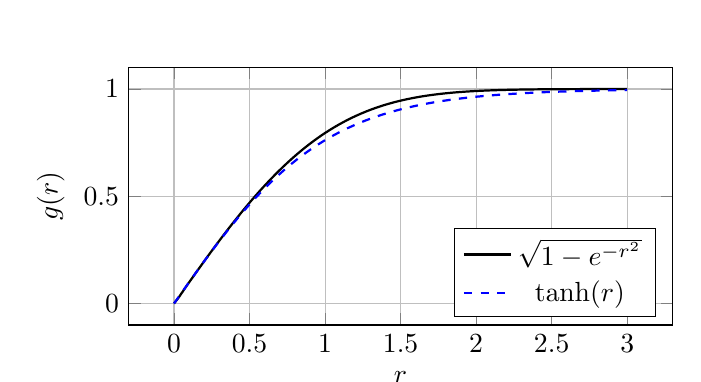
\begin{tikzpicture}
    \begin{axis}[
        xlabel={$r$},
        ylabel={$g(r)$},
        legend pos=south east,
        grid=both,
        width=0.7\textwidth,
        height=0.4\textwidth,
      ]
      \addplot[
        domain=0:3,
        samples=100,
        black,
        thick,
      ] {sqrt(1 - exp(-x^2))};
      \addlegendentry{$\sqrt{1 - e^{-r^2}}$}
      \addplot[
        domain=0:3,
        samples=100,
        blue,
        dashed,
        thick,
      ] {tanh(x)};
      \addlegendentry{$\tanh(r)$}
    \end{axis}
  \end{tikzpicture}
  \caption{Comparison of $g(r) = \tanh(r)$ and $g(r) = \sqrt{1 - e^{-r^2}}$.}
  \label{fig:radial-transformations}
\end{figure}

This particular formulation has the advantage of simplifying the Poincaré distance expression in \eqref{eq:poincare-distance}. Namely, let $y_i = f(x_i)$ be the output of the MLP, and consider computing the Poincaré distance between output vectors \emph{normalized} via $g$.\footnote{Abusing notation, we will let $g(y_i)$ denote a \emph{vector} that is in the direction of $y_i$ but with norm equal to $g(\norm{y_i})$.} The quantity in the denominator simplifies through $1 - \norm{g(y_i)}^2 = e^{-\norm{y_i}^2}$. The Poincaré metric---accounting for normalization---is then\footnote{In practice, we must also add a small $10^{-7}$ epsilon to the argument of $\text{arcosh}(\cdot)$ to avoid numerical issues.}
\begin{align}
  \sigma(y_i, y_j)
  = d \Big( g(y_i), g(y_j) \Big)
  = \text{arcosh} \qty[1 + 2 \frac{\norm{g(y_i) - g(y_j)}^2}{e^{-\norm{y_i}^2} e^{-\norm{y_j}^2}}] \; .
\end{align}

\begin{figure}[H]
  \centering
  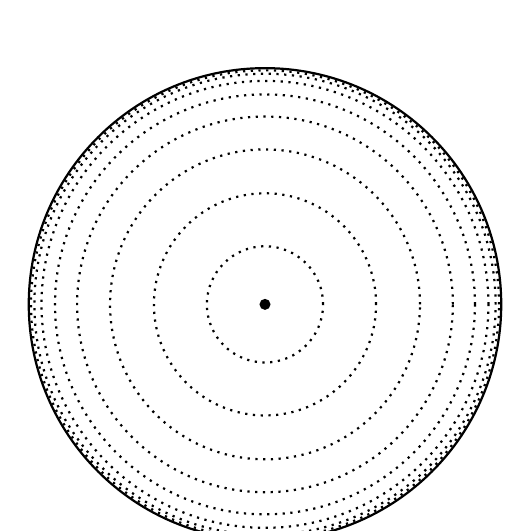
\begin{tikzpicture}
    % Draw the unit circle (Poincaré disk boundary)
    \draw[thick] (0,0) circle (3);
    % Draw level curves at every 0.25 (pre-transformed)
    \draw[thick, dotted] (0,0) circle (0.738);
    \draw[thick, dotted] (0,0) circle (1.411);
    \draw[thick, dotted] (0,0) circle (1.968);
    \draw[thick, dotted] (0,0) circle (2.386);
    \draw[thick, dotted] (0,0) circle (2.667);
    \draw[thick, dotted] (0,0) circle (2.838);
    \draw[thick, dotted] (0,0) circle (2.929);
    \draw[thick, dotted] (0,0) circle (2.972);
    % Draw the origin
    \fill (0,0) circle (0.07);
  \end{tikzpicture}
  \caption{Level curves in the Poincaré disk at normalized radii $g(0.25), g(0.5), \dots, g(2.0)$.}
  \label{fig:poincare-level-curves}
\end{figure}

\subsection{Poincaré Metric Scale Parameter}

In addition, when training the embedding function, we learn a \emph{scale parameter} $\texttt{SCALE} \geq 0$ that governs the global scale of the hyperbolic metric. That is, the actual distance used is
\begin{align}
  \texttt{SCALE} * \sigma(y_i, y_j)
\end{align}

A larger scale parameter \texttt{SCALE} keeps the points closer to the origin on the disk, and vice versa. When training, we observe that the scale starts decreasing and points start being pushed away from the origin to compensate. This is usually a good thing: the embeddings start leveraging the edge of the disk, where there is more \emph{space} to fit tree-like structures. However, computing distances of points too close to the boundary leads to numerical issues, so we lower-bound the scale parameter to avoid this issue.

\section{Methodology}

We propose a novel method that takes as input an arbitrary set of computer files and organizes them into a nested tree of directories. Example repositories containing files in a hierarchical directory structure are used to train a ``generative'' model that can then organize unseen files.

Our method consists of three parts:

\begin{enumerate}
  \item Map files to feature vectors with the help of a pre-trained LLM. Namely, given a file $u_i$, the feature vector $x_i = \phi(u_i)$ should capture useful semantic information about the file. There are no learned parameters in this part.
  \item Learn a function $f$ that embeds file feature vectors into a low-dimensional metric space $(Y, \sigma)$. The mapping should preserve the true tree distance between files with low distortion. We experiment with Euclidean and hyperbolic target spaces. We take $f$ to be a multi-layer perceptron.
  \item Organize a given set of files $\qty{u_1, u_2, \dots}$ hierarchically, with the end goal of creating a directory tree containing the files (physically, on disk). New/unseen files are feature expanded via $\phi$ and embedded into $(Y, \sigma)$ using the learned function $f$. Hierarchical clustering is then performed on the embedded files to create the directory tree.
\end{enumerate}

\begin{figure}[H]
  \begin{align*}
    \begin{Bmatrix}
      \texttt{file1.ext} \\
      \texttt{file2.ext} \\
      \vdots             \\
      \texttt{fileN.ext}
    \end{Bmatrix}
    \xrightarrow{\text{fixed LLM}}
    \begin{Bmatrix}
      \langle \dots \text{features} \dots \rangle_1 \\
      \langle \dots \text{features} \dots \rangle_2 \\
      \vdots                                        \\
      \langle \dots \text{features} \dots \rangle_N
    \end{Bmatrix}
    \xrightarrow{\text{MLP}}
    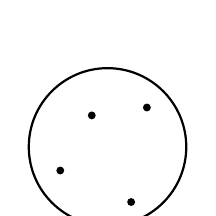
\begin{tikzpicture}[baseline={(0,-0.1)}]
      % unit circle
      \draw[thick] (0,0) circle (1);
      % some points
      \fill (0.5,0.5) circle (0.05);
      \fill (-0.2,0.4) circle (0.05);
      \fill (0.3,-0.7) circle (0.05);
      \fill (-0.6,-0.3) circle (0.05);
    \end{tikzpicture}
    \xrightarrow{\text{h-clustering}}
    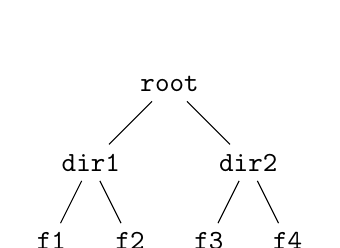
\begin{tikzpicture}[baseline={(0,-1.1)}]
      % tree nodes
      \node (root) at (0,0) {\texttt{root}};
      \node (dir1) at (-1,-1) {\texttt{dir1}};
      \node (dir2) at (1,-1) {\texttt{dir2}};
      \node (file1) at (-1.5,-2) {\texttt{f1}};
      \node (file2) at (-0.5,-2) {\texttt{f2}};
      \node (file3) at (0.5,-2) {\texttt{f3}};
      \node (file4) at (1.5,-2) {\texttt{f4}};
      % tree edges
      \draw (root) -- (dir1);
      \draw (root) -- (dir2);
      \draw (dir1) -- (file1);
      \draw (dir1) -- (file2);
      \draw (dir2) -- (file3);
      \draw (dir2) -- (file4);
    \end{tikzpicture}
  \end{align*}
  \caption{High-level flow chart of \textsc{Forg}.}
\end{figure}

\subsection{Summary of Notation}

Below is a summary of the notation that is used throughout the rest of the report:

\begin{itemize}
  \item $u_i \in U$: a file from the space of all files.
  \item $U_\text{train}, U_\text{test} \subset U$: the set of training and test files, respectively.
  \item $\mathcal T(u_i, u_j)$: the true file tree distance between training files $u_i, u_j \in U_\text{train}$. Note that $(U_\text{train}, \mathcal T)$ forms a metric space.
  \item $d$: the dimensionality of the feature vectors.
  \item $D$: the dimensionality of the target metric space.
  \item $x_i \in X = \mathbb{R}^d$: the feature vector of file $u_i$.
  \item $\phi: U \to X$: a fixed function that maps files to feature vectors.
  \item $f: X \to Y$: a learned function that embeds file feature vectors into a metric space, preserving distances.
  \item $(Y, \sigma)$: the target metric space in which we perform hierarchical clustering of files. For Euclidean spaces, we write $Y = \mathbb R^D$. For hyperbolic spaces, we write $Y = \mathcal H^D$.
  \item $\Sigma^*$: the set of all strings, formed from a standard alphabet $\Sigma$.
\end{itemize}

\subsection{Part 1: Mapping Files to Feature Vectors}

Let $U$ be the space of all files. We start by defining a fixed, deterministic mapping $\phi: U \to X$ that maps files into $d$-dimensional feature vectors ($X = \mathbb R^d$). These file features should be suitable for downstream file embedding and clustering tasks. Specifically, for a given file, we are interested in properties that correlate with its location in the file system tree.

Let $\Sigma$ be the set of characters in a standard alphabet, e.g., ASCII ($\abs{\Sigma} = 128$), or more generally, Unicode. Let $\Sigma^*$ denote the infinite set of all character strings. In our case, we look at a file's name and contents, ignoring other metadata like creation date and owner. These properties should correlate with a file's position in the file tree.

Given a file $u_i \in U$, we denote these properties as $\textsc{Filename}_i \in \Sigma^*$ and $\textsc{Contents}_i \in \Sigma^*$. (We will deal with non-text files later.) We create a \emph{string-to-feature} function $\phi_s: \Sigma^* \to \mathbb R^{d/2}$, such that the overall file feature vector is given by following concatenation:
\begin{align}
  \phi(u_i) =
  \Big(\phi_s(\textsc{Filename}_i), \phi_s(\textsc{Contents}_i) \Big) \in \mathbb R^d \; .
\end{align}

We propose two constructions of $\phi_s$, the string-to-feature function.

\subsubsection{String-to-Feature Construction 1: Counts of Top Tokens}

Let $s \in \Sigma^*$ be the input string to $\phi_s$. Furthermore, we consider the top $t$ tokens of the pre-trained LLM's tokenizer.\footnote{Roughly speaking, these tokens are the $t$ most frequently seen $n$-grams during the LLM's training. Given no other \emph{a priori} information about file contents, we believe relying on a pre-trained tokenizer (which has been fitted on vast sums of internet text) is a reasonable way to discretize input strings.} We then compute
\begin{align}
  \phi_s(s) = \Big( \text{count}_1(s), \text{count}_2(s), \dots, \text{count}_t(s) \Big) \; ,
\end{align}
where $\text{count}_i(s)$ is the number of times the $i$-th most frequent token appears in the tokenized version of $s$. This construction yields $d = 2t$.

Roughly, this approach captures an intuition that token counts capture enough semantic meaning to be useful for predicting file system tree distances.

\subsubsection{String-to-Feature Construction 2: Last Hidden State of LLM}

We can also use the last hidden state of the LLM as the feature vector. This is a common practice in NLP, as the last hidden state is thought to contain a compressed representation of the input text. Namely, our LLMs have been pre-trained over vast sums of text such that the last hidden state represents the input text in a way that is useful for next-token prediction.

In general, if $d_k$ is the token embedding dimension of the LLM, and $\abs{s}$ is the number of tokens in $s$, then the last hidden state is a $\mathbb R^{\abs{s} \times d_k}$ matrix. It contains the \emph{refined} $d_k$-dimensional embedding of each input token. We try two different approaches to produce the final feature vector:
\begin{enumerate}
  \item Average the token embeddings across the $\abs{s}$ tokens.
  \item Take the embedding of the last token. The idea behind this strategy is that by the time the input has passed through the various self-attention layers, the last token's embedding has been adjusted to incorporate information from preceding tokens. When using the last token embedding, we can employ the \emph{Explicit One word Limitation (PromptEOL)} strategy described in \cite{jiang2023scalingsentenceembeddingslarge}, where we wrap the input \texttt{string} in the template:
        \begin{center}
          \texttt{This file content: " [string] " contains in one word: "}
        \end{center}
        This strategy has been shown to improve the relevance of the last token embedding.
\end{enumerate}

A potential concern is that the distribution of \textsc{Filename} and \textsc{Contents} strings are, in general, quite different from the natural language text that LLMs are trained on. Still, we believe that tokenization and subsequent embedding capture interesting details. For \textsc{Filename}, we may want to identify strings like \texttt{foo-test.js} and \texttt{bar-test.js}, which correspond files in the same \texttt{src/\_\_tests\_\_} directory. Both names may contain the shared tokens \texttt{["test", ".js"]}, so passing the names through the LLM should produce similar hidden state embeddings. Similarly, for \textsc{Contents}, HTML files may contain many \texttt{<div>} tokens, and these tokens should have similar influences on the hidden state.

At minimum, the hidden state can be seen as capturing info similar to the token counts in the previous construction.

\subsubsection{Feature Vectors for Non-Text Files}

For non-text (i.e., binary) files, we learn a global feature vector $c^* \in \mathbb{R}^{d/2}$ to use in place of $\phi_s(\text{CONTENTS}_i)$ encoding file content tokens. In particular, for any binary file $u_i$, we learn a $c^*$ such that
\begin{align}
  \phi(u_i) = \Big(\phi_s(\textsc{Filename}_i), c^*\Big) \in \mathbb{R}^d
\end{align}

\subsection{Part 2: Learning the Embedding Function}

This part learns an approximately-distance-preserving embedding function $f: X \to Y$ that embeds the feature vectors into a low-dimensional metric space $(Y, \sigma)$. The embedding model is optimized over a set of training files $U_\text{train} \subset U$, which exist in a known file system tree. Thus, the true tree distance $\mathcal T(u_i, u_j)$ is known between all files. Of course, we first compute $x_i = \phi(u_i) \in X$ for each training file, which becomes the input to $f$. The embedding function $f$ that we choose takes the form of a multi-layer perceptron (MLP) with two hidden layers, each with width=512 nodes, with ReLU activation applied to each intermediate output.

The goal is to minimize the discrepancy between the true tree distance $\mathcal T$ and the distance in the target metric space $\sigma$. We study two different cost functions that quantify this distance discrepancy.

\subsubsection{Cost Function 1: Mean Squared Error}

The obvious strategy is to minimize the mean squared error of distances between all $\abs{U_\text{train}}^2$ pairs of files. Namely, we minimize the following expression with respect to the parameters of $f$ using the ADAM optimizer:
\begin{align}
  \sum_{(u_i, u_j) \in U_\text{train}^2} \Big[ \sigma(f(\phi(u_i)), f(\phi(u_j)) - \mathcal T(u_i, u_j) \Big]^2 \; .
  \label{eq:mse-cost}
\end{align}

\subsubsection{Cost Function 2: t-SNE Objective}

We may also want to prioritize preserving local distances, rather than giving equal weight to all $\abs{U_\text{train}}^2$ distances. We can instead optimize the t-SNE cost function presented in \cite{maaten2008visualizing}:
\begin{align}
  \sum_i KL(P||Q) = \sum_i \sum_j p_{ij} \log \frac{p_{ij}}{q_{ij}} \; .
  \label{eq:tsne-cost}
\end{align}

The $P$ and $Q$ distributions follow the standard form, as in \cite{maaten2008visualizing}. Notably, $p$ is defined with respect to tree distance $\mathcal T$, and $q_{ij}$ is defined with respect to embeddings $f(\phi(u_i))$ in the target space.

\subsection{Part 3: Organizing Files Hierarchically}

Finally, we propose a procedure to organize files hierarchically. Here, we consider ``test'' files $U_\text{test} \subset U$ whose true tree distances are unknown. These files have not been used to train the embedding function $f$.

Using the fixed feature expansion and learned embedding function, we can embed each test file into the target space $(Y, \sigma)$. Namely, we compute $y_i = f(\phi(u_i))$ for all $u_i \in U_\text{test}$.

Then, we utilize standard agglomerative hierarchical clustering methods to organize the embedded files into a tree. Our method supports the various clustering schemes listed in \cite{müllner2011modernhierarchicalagglomerativeclustering}, including \texttt{single}, \texttt{complete}, and \texttt{Ward}. We use \texttt{scipy.cluster.hierarchy.linkage} from SciPy to perform the clustering. The resulting tree is used to produce a directory structure in which the files are then placed.

The user specifies a \texttt{num\_dirs} parameter (e.g., 10) that specifies exactly how many directories are to appear in the final directory hierarchy. The top \texttt{num\_dirs} longest edges in the cluster tree are ``cut''; at each cut, a new directory is created to contain the subtree.

\begin{figure}[H]
  \centering
  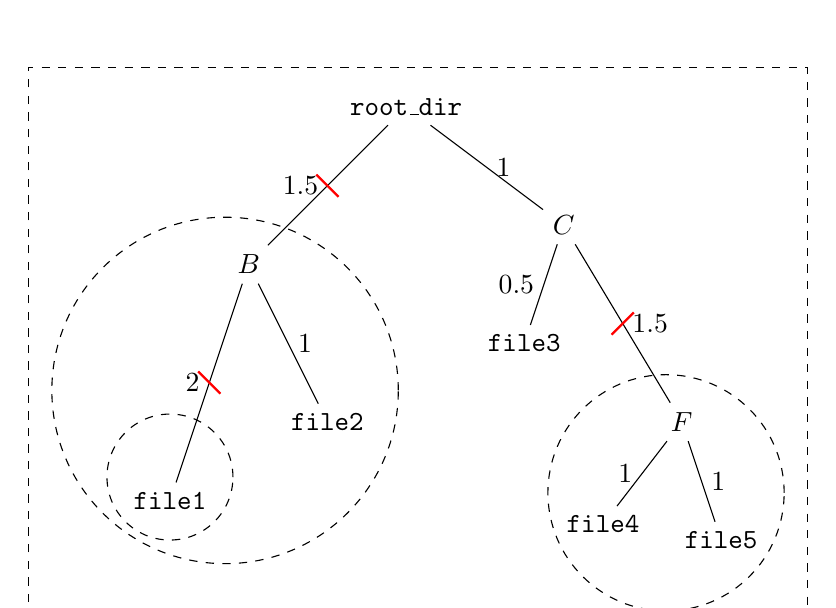
\begin{tikzpicture}
    % Define nodes
    \node (A) at (0,0) {\texttt{root\_dir}};
    \node (B) at (-2,-2) {$B$};
    \node (C) at (2,-1.5) {$C$};
    \node (D) at (-3,-5) {\texttt{file1}};
    \node (E) at (-1,-4) {\texttt{file2}};
    \node (F) at (3.5,-4) {$F$};
    \node (G) at (1.5,-3) {\texttt{file3}};
    \node (H) at (2.5,-5.3) {\texttt{file4}};
    \node (I) at (4,-5.5) {\texttt{file5}};

    % Draw edges with varying lengths
    \draw (A) -- node[midway, left] {$1.5$} (B);
    \draw (A) -- node[midway, right] {$1$} (C);
    \draw (B) -- node[midway, left] {$2$} (D);
    \draw (B) -- node[midway, right] {$1$} (E);
    \draw (C) -- node[midway, right] {$1.5$} (F);
    \draw (C) -- node[midway, left] {$0.5$} (G);
    \draw (F) -- node[midway, left] {$1$} (H);
    \draw (F) -- node[midway, right] {$1$} (I);

    % Cut the top 3 longest edges
    % Edges: (A)-(B), (B)-(D), (C)-(F)
    \draw[red, thick] ($(A)!0.5!(B)$) -- ++(135:0.2) -- ++(-45:0.4);
    \draw[red, thick] ($(B)!0.5!(D)$) -- ++(135:0.2) -- ++(-45:0.4);
    \draw[red, thick] ($(C)!0.5!(F)$) -- ++(45:0.2) -- ++(-135:0.4);

    % Draw circles around subtrees in new directories
    \draw[dashed] (-2.3,-3.6) circle (2.2);
    \draw[dashed] (-3.0,-4.7) circle (0.8);
    \draw[dashed] (3.3,-4.9) circle (1.5);

    % Surround whole tree in a rectangle
    \draw[dashed] (-4.8,-6.5) rectangle (5.1,0.5);

  \end{tikzpicture}
  \caption{A tree with varying branch lengths. The top three longest edges are cut to create new directories (shown in dashed lines).}
  \label{fig:example-tree-with-cuts}
\end{figure}

\begin{figure}[H]
  \centering
  \begin{BVerbatim}
    root_dir
    ├── dir1
    │   ├── dir2
    │   │   └── file1
    │   └── file2
    ├── dir3
    │   ├── file4
    │   └── file5
    └── file3
  \end{BVerbatim}
  \caption{The directory structure produced from the tree in Figure \ref{fig:example-tree-with-cuts}.}
  \label{fig:example-directory-structure}
\end{figure}

\subsection{Time Complexity Analysis}

Empirically, the amount of time it takes to compute the embeddings $\phi(u_i)$ is dominated by how long it takes the LLM to embed the filename and content tokens, and the specific runtime is proportional to the number of tokens in $u_i$ and is LLM-dependent. However, when running multiple experiments on the same data, we can cache the embeddings, significantly speeding up this step of our procedure.

For each training epoch, the embedding distortion objective \eqref{eq:mse-cost} takes $O(\abs{U_\text{train}}^2)$ to evaluate because it sums over all pairs of files. To reduce runtime here, we randomly sample a subset of files to both train on and evaluate the objective over, with the number of files \texttt{SAMPLES} given as a user-provided input. Thus, the entire training step takes $O(\text{\# of epochs} \cdot \abs{U_\text{train}}^2)$ time to complete.

Finally, performing agglomerative clustering using the SLINK algorithm \cite{sibson1973slink} has a time complexity of $O(\abs{U_\text{test}}^2)$, and reconstructing a file directory hierarchy from this takes $O(\abs{U_\text{test}} \cdot \texttt{num\_dirs})$ time using naive search.

\section{Experiments}

We evaluate our method's performance in the context of organizing files from GitHub repositories. We focus on React, an MIT-licensed JavaScript library built by Meta for building user interfaces. We chose this repository because React is one of the most popular libraries among developers. Furthermore, the repository contains a variety of file types, organized according to good practices.

The React repository has $N=6922$ total files. In our experiments, we randomly select 3000 files using a fixed seed, then partition them into 80\% training data and 20\% test data. We analyze the test cost across training epochs, using the MSE formulation in \eqref{eq:mse-cost}. In our experiments, we know the true tree distances between test files, which lets us compute the test cost. All runs were performed using Google's Gemma 2B LLM for feature expansion, unless otherwise noted.

We find that the convergence of Hyperbolic embeddings is quite sensitive to learning rate. Using the Adam optimizer, the learning rate must be within the realm of $10^{-4}$.

\subsection{Testing on Various Repositories}

Before focusing on React, we run our method on the various repositories listed in Table \ref{tab:repositories}. We observe that the test cost decreases across epochs, indicating that the learned MLP is able to generalize. However, as shown in Figure \ref{fig:basic-test-costs}, the test cost during training is somewhat sensitive to the random initialization of the MLP weights. Across five runs, the minimum and maximum test costs across epochs differ by roughly 1. For each repository, we sample 3000 files, partitioning them into 80\% training data and 20\% test data.

\begin{table}[H]
  \centering
  \begin{tabular}{lcr}
    \toprule
    \textbf{Repository} & \textbf{\# of Files} & \textbf{Min Test Cost} \\
    \midrule
    React               & 6922                 & $6.704 \pm 0.265$      \\
    PyTorch             & 85767                & $4.64 \pm 0.143$       \\
    \texttt{/var}       & 5919                 & $0.7166 \pm 0.0407$    \\
    \bottomrule
  \end{tabular}
  \caption{We test our method on three repositories. For React, dependencies (\texttt{node\_modules}) are \emph{excluded}. For PyTorch, dependencies (Git submodules) are \emph{included}. \texttt{/var} refers to the \texttt{/var} directory in a fresh Ubuntu 22.04 LTS installation. We use the main branches of the React and PyTorch repositories, cloned in November 2024.}
  \label{tab:repositories}
\end{table}

\begin{figure}[H]
  \begin{minipage}{0.33\textwidth}
    \centering
    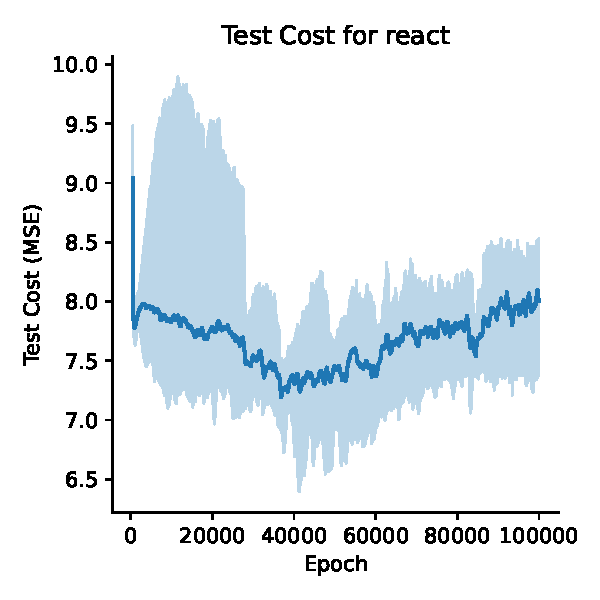
\includegraphics[width=\linewidth]{figures/basic_test_cost_react.pdf}
  \end{minipage}%
  \begin{minipage}{0.33\textwidth}
    \centering
    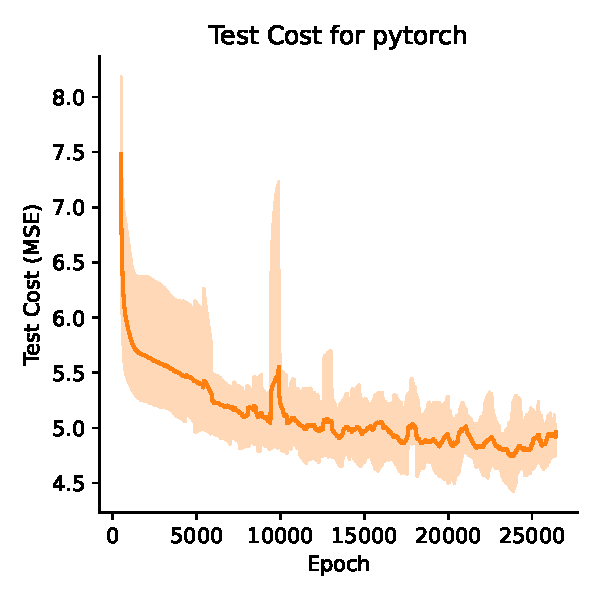
\includegraphics[width=\linewidth]{figures/basic_test_cost_pytorch.pdf}
  \end{minipage}%
  \begin{minipage}{0.33\textwidth}
    \centering
    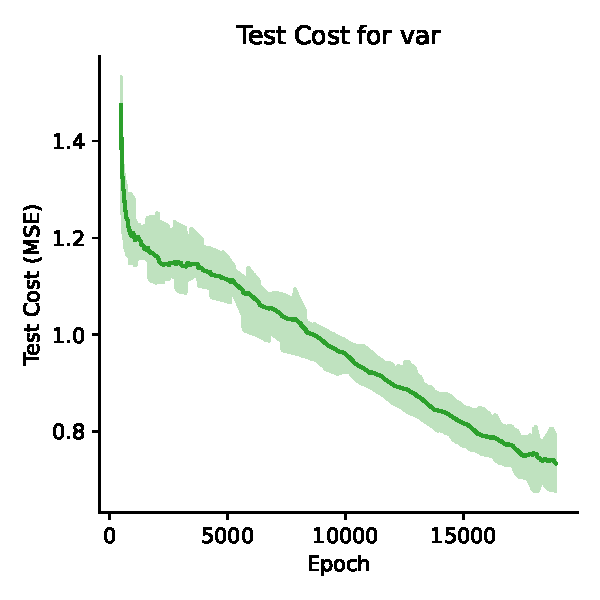
\includegraphics[width=\linewidth]{figures/basic_test_cost_var.pdf}
  \end{minipage}
  \caption{Test costs across training epochs for React, PyTorch, and the Ubuntu \texttt{/var} directory. The test costs decrease across epochs, indicating that the learned MLP is able to generalize. The shaded region represents the minimum and maximum test costs across five runs. These runs use the hyperbolic metric with $D=2$. The test cost is especially low for \texttt{/var}, possibly because the directory structure is flatter.}
  \label{fig:basic-test-costs}
\end{figure}

\subsection{Double Descent}

We observe a double descent phenomenon in the test cost, which is especially pronounced under the hyperbolic metric. Figure \ref{fig:metric-and-dimensionality-short-term} shows that the test cost reaches a minimum after a few hundred epochs. We call this the \emph{short-term} behavior. However, after a few orders of magnitude more epochs, the test cost starts to decrease again. We call this the \emph{long-term} behavior, as shown in Figure \ref{fig:metric-and-dimensionality-long-term}. After about 20K--100K epochs, the test cost reaches a new minimum.

In the hyperbolic case, the long-term minimum is lower than the short-term minimum. We believe this is due to the fact that gradually, the MLP learns to embed files towards the edge of the Poincaré disk, where there is more \emph{space} to fit tree-like structures. In tandem, the \texttt{SCALE} parameter decreases over time to compensate for the increased distance between points. This effect is shown in Figure \ref{fig:short-and-long-term-embeddings}.

\subsection{Effect of Metric and Dimensionality}

We find concrete evidence that embedding into a hyperbolic space produces lower test costs than embedding into a Euclidean space. In the short term, this difference is not noticeable because the embeddings start near the origin of the Poincaré disk (see Figure \ref{fig:metric-and-dimensionality-short-term}). However, in the long term, as the embeddings move towards the boundary of the disk, the hyperbolic embeddings outperform the Euclidean embeddings (see Figure \ref{fig:metric-and-dimensionality-long-term}).

We also find that higher dimensionality spaces lead to lower test costs, for both Euclidean and hyperbolic metrics. This is likely because higher dimensionality spaces also give more \emph{space} to fit tree-like structures. However, as seen in Figure \ref{fig:metric-and-dimensionality-long-term}, even a high-dimensional $D=6$ Euclidean space is outperformed by a $D=2$ hyperbolic space. Going into higher dimensions in hyperbolic space provides additional benefits, but with diminishing returns.

\begin{figure}[H]
  \centering
  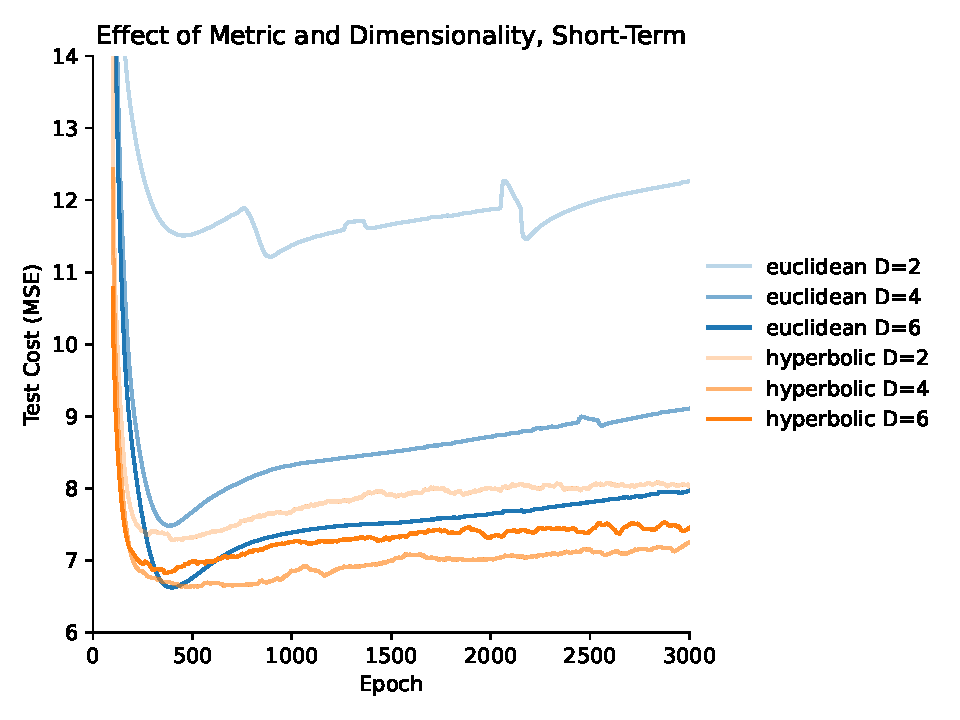
\includegraphics[width=0.7\textwidth]{figures/metric_and_dimensionality_short_term.pdf}
  \caption{These are the test loss curves across Euclidean and hyperbolic metrics, with varying dimensionality. The test losses reach an initial minimum after a few hundred epochs. In the short term, there is no distinct difference between Euclidean and hyperbolic metrics.}
  \label{fig:metric-and-dimensionality-short-term}
\end{figure}

\begin{figure}[H]
  \centering
  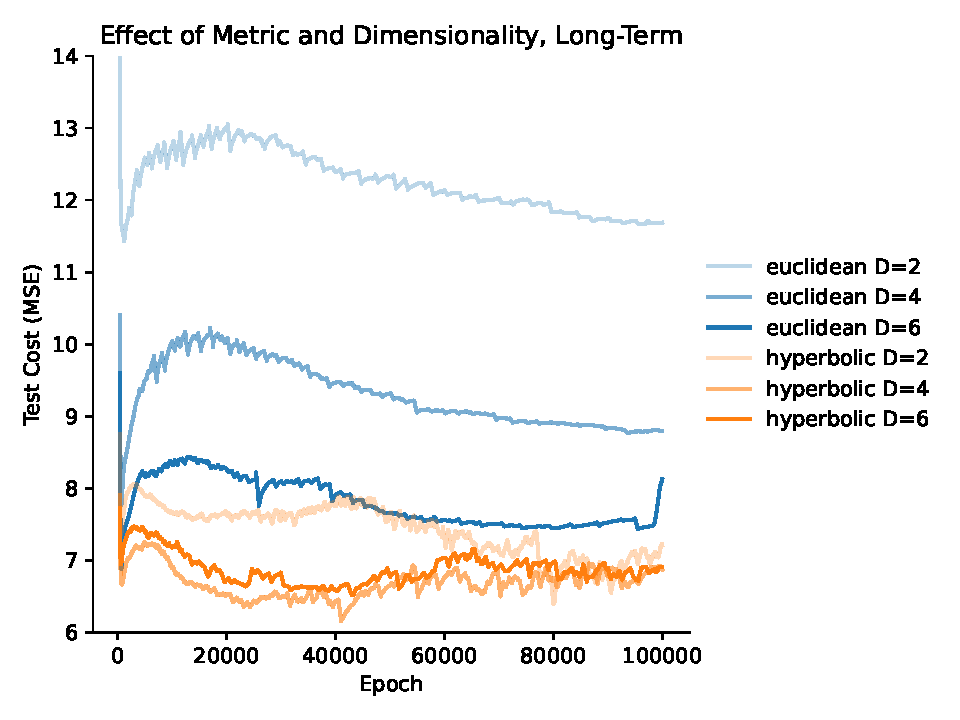
\includegraphics[width=0.7\textwidth]{figures/metric_and_dimensionality_long_term.pdf}
  \caption{In the long term (tens of thousands of epochs), the test losses reach a new minimum. For the hyperbolic metric, the long-term minimum is lower than the short-term minimum. Increasing the dimensionality of the target space leads to lower test costs, but the effect is less pronounced in the hyperbolic case.}
  \label{fig:metric-and-dimensionality-long-term}
\end{figure}

\begin{figure}[H]
  \centering
  \begin{minipage}{0.35\textwidth}
    \centering
    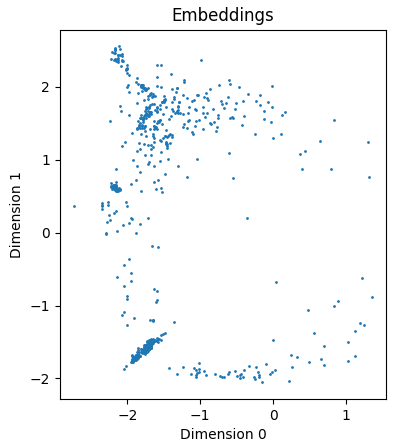
\includegraphics[width=\linewidth]{figures/short_term.png}
  \end{minipage}%
  \begin{minipage}{0.35\textwidth}
    \centering
    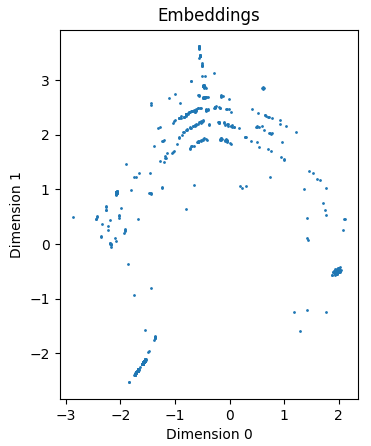
\includegraphics[width=\linewidth]{figures/long_term.png}
  \end{minipage}
  \caption{Comparison of Poincaré embeddings in the short term (left) and long term (right). The embeddings are plotted pre-normalization (using $g$), which explains why their norms are not bounded to $[0, 1)$. Recall that embeddings larger than $1$ are ``smoothly compressed'' into the Poincaré disk. This means that in the long-term plot, the normalized embeddings are very close to the boundary of the disk.}
  \label{fig:short-and-long-term-embeddings}
\end{figure}

\subsection{Effect of Feature Expansion of Files}

We analyze the performance with respect to the choice of LLM used in the feature expansion $\phi$. We find that pre-trained LLMs with higher parameter counts produce feature expansions that lead to lower test costs. This makes sense: larger LLMs have been trained on more data and produce embeddings that better capture the semantics of the input strings. See Figure \ref{fig:expansion-model} for a comparison of Google's Gemma 2B and Meta's Llama 3 8B.

\begin{figure}[H]
  \centering
  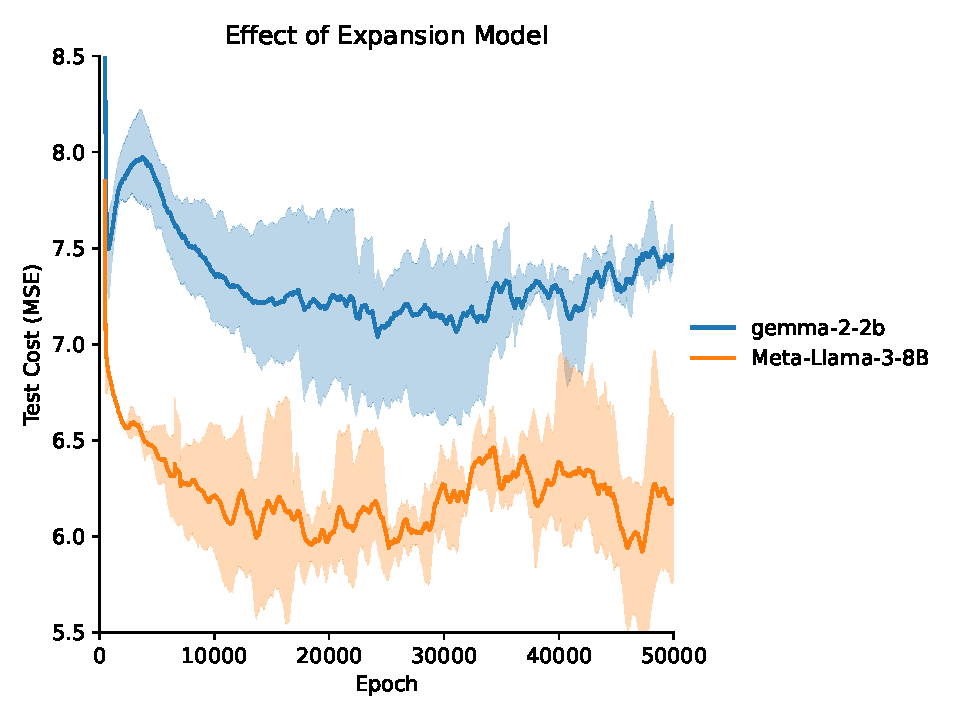
\includegraphics[width=0.7\textwidth]{figures/expansion_model.pdf}
  \caption{Comparison of using different LLMs for feature expansion. We use the 8B-parameter Llama 3 model from Meta and the 2B-parameter Gemma model from Google. The 8B-parameter model produces lower test costs. The curves show the min, max, and mean costs across three runs.}
  \label{fig:expansion-model}
\end{figure}

Furthermore, we benchmark the various string-to-feature constructions $\phi_s$ (i.e., how to interpret the LLM's hidden state). We find that simply taking the average of the token embeddings across all input tokens produces the best feature vectors. When choosing to use just the last token embeddings, however, the \emph{PromptEOL} strategy from \cite{jiang2023scalingsentenceembeddingslarge} still gives a measurable boost in performance.

\begin{figure}[H]
  \centering
  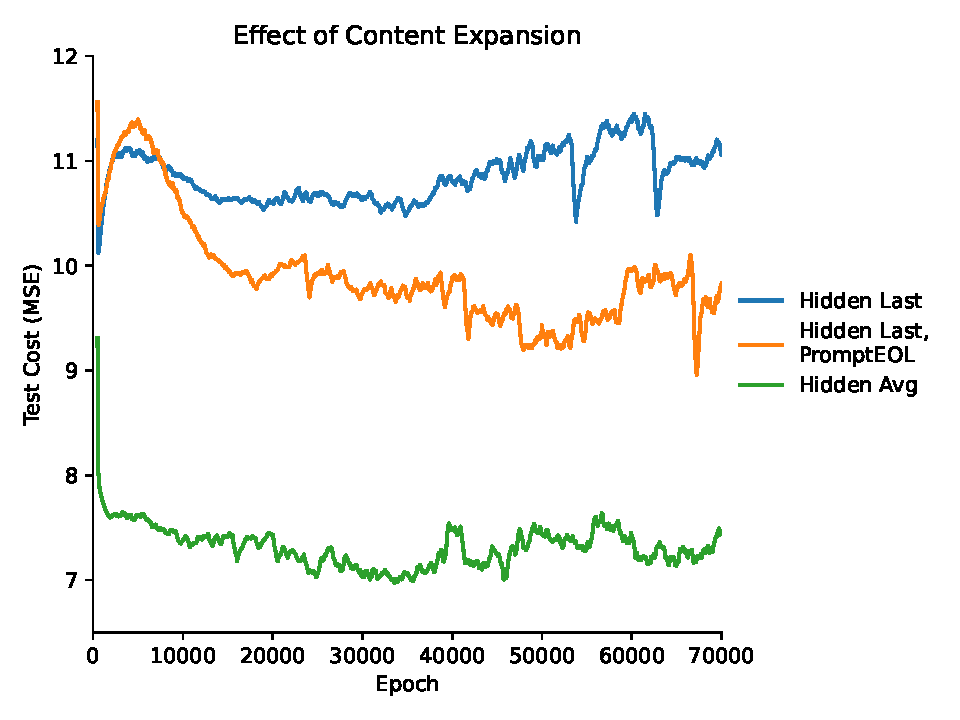
\includegraphics[width=0.7\textwidth]{figures/content_expansion.pdf}
  \caption{Comparison of different string-to-feature constructions $\phi_s$. Simply averaging the entire final hidden state produces the best feature vectors. Still, the \emph{PromptEOL} strategy from \cite{jiang2023scalingsentenceembeddingslarge} is useful when using just the last token embedding.}
  \label{fig:content-expansion}
\end{figure}

\subsection{Qualitative Analysis}

We qualitatively analyze the embeddings produced by our method. Figure \ref{fig:React-training-and-test-embeddings} shows that the learned embedding function indeed groups together files from key top-level directories in the React repository.

\begin{figure}[H]
  \begin{minipage}{0.5\textwidth}
    \centering
    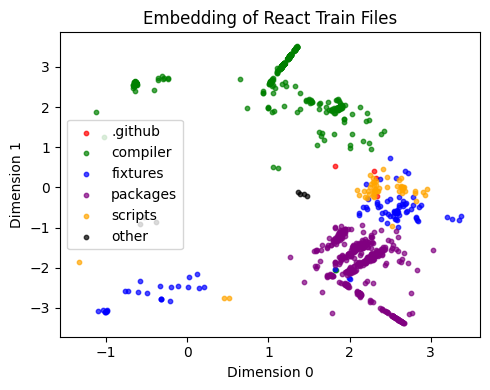
\includegraphics[width=\linewidth]{figures/react_train.png}
  \end{minipage}%
  \begin{minipage}{0.5\textwidth}
    \centering
    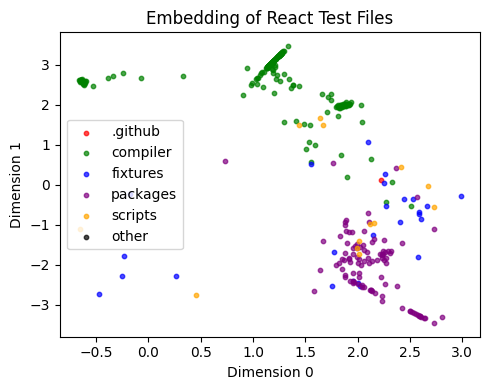
\includegraphics[width=\linewidth]{figures/react_test.png}
  \end{minipage}
  \caption{Visualization of how hyperbolic embeddings of files from the six primary directories in the React repository cluster together. The right plot shows that the embedding function learns to group together files from the same directory, even for unseen test files.}
  \label{fig:React-training-and-test-embeddings}
\end{figure}

We also look at the qualitative differences in embeddings produced by the MSE and t-SNE cost functions. As expected, the t-SNE cost function produces ``cluster-happy'' embeddings (see figure \ref{fig:cost-function-emnbeddings}). However, we find that the MSE cost function produces embeddings that are more suitable for hierarchical clustering.

\begin{figure}[H]
  \begin{minipage}{0.5\textwidth}
    \centering
    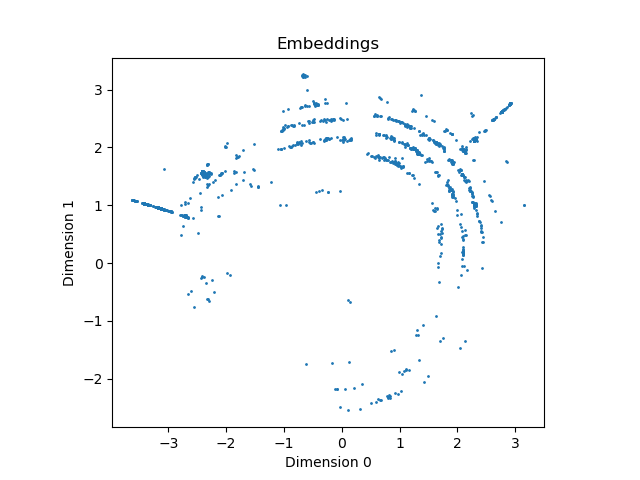
\includegraphics[width=\linewidth]{figures/mse_cost.png}
  \end{minipage}%
  \begin{minipage}{0.5\textwidth}
    \centering
    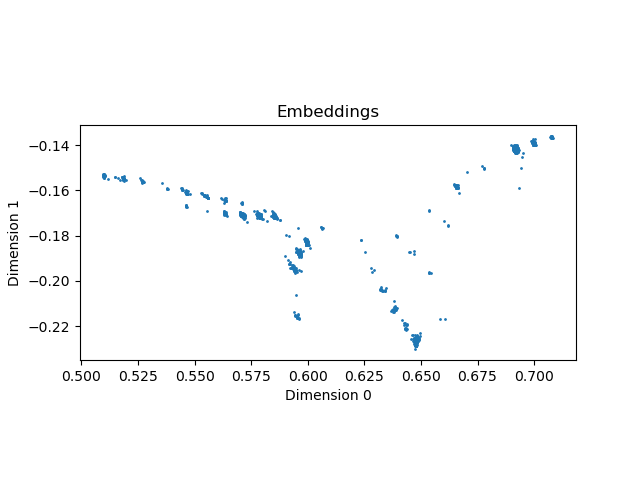
\includegraphics[width=\linewidth]{figures/tsne_cost.png}
  \end{minipage}
  \caption{Comparison of (pre-normalization) hyperbolic embeddings produced by the MSE (left) and t-SNE (right) cost functions. In the MSE case, the embeddings are organized into distinct rings, which reflects the hierarchical structure of the file system tree. In the t-SNE case, higher importance is given to local structure, leading to \emph{islands} of embeddings.}
  \label{fig:cost-function-emnbeddings}
\end{figure}

\subsection{Transfer Learning}

We take the embedding model $f$ trained on the React repository and apply it to the \textsc{Forg} repository (i.e., the very code used in all these experiments). The resulting file tree in figure \ref{fig:forg-directory-structure} shows that the model produces a very reasonable directory structure (keep in mind that it was trained on a JavaScript repository and applied to a Python repository).

\begin{figure}[H]
  \centering
  % \begin{noindent}
  \begin{BVerbatim}
    [root]
    ├── [dir]
    │   ├── [dir]
    │   │   └── embedding_metric.cpython-312.pyc
    │   ├── [dir]
    │   │   └── costs.cpython-312.pyc
    │   ├── [dir]
    │   │   └── tree_metric.cpython-312.pyc
    │   ├── [dir]
    │   │   └── feature.cpython-312.pyc
    │   ├── __init__.cpython-312.pyc
    │   ├── [dir]
    │   │   └── embedding_cache.cpython-312.pyc
    │   ├── [dir]
    │   │   └── file.cpython-312.pyc
    │   ├── cluster.cpython-312.pyc
    │   ├── embedding.cpython-312.pyc
    │   ├── metric.cpython-312.pyc
    │   ├── train.cpython-312.pyc
    │   └── utils.cpython-312.pyc
    └── [dir]
        ├── __init__.py
        ├── cluster.py
        ├── costs.py
        ├── embedding.py
        ├── embedding_cache.py
        ├── embedding_metric.py
        ├── feature.py
        ├── file.py
        ├── train.py
        ├── tree_metric.py
        └── utils.py
  \end{BVerbatim}
  % \end{noindent}
  \caption{The directory structure produced by the model when applied to the \textsc{Forg} repository (Ward linkage, \texttt{num\_dirs=7}). The model was trained on the React repository. Observe that the model correctly separates \texttt{.py} source files and \texttt{.pyc} compiled files.}
  \label{fig:forg-directory-structure}
\end{figure}

We also study the model's performance when trained on a historical snapshot of the React repository and applied to the current React repository. This is important because we may want to tune a model to a specific repository, and expect it to perform well even as the repository evolves. Table \ref{tab:historical-transfer} shows that the model's performance degrades as the gap between the training and test years increases.


\begin{table}[H]
  \centering
  \begin{tabular}{lcr}
    \toprule
    \textbf{Training Year} & \textbf{\# of Training Files} & \textbf{Test Cost} \\
    \midrule
    2016                   & 940                           & 42.205             \\
    2018                   & 801                           & 47.745             \\
    2020                   & 1673                          & 27.114             \\
    2022                   & 2424                          & 23.853             \\
    \bottomrule
  \end{tabular}
  \caption{Performance of the model when trained on historical snapshots of the React repository (earliest major release in each indicated year) and evaluated on the current React repository (December 2024). The MSE test cost is larger when more years of change have occurred between training and testing.}
  \label{tab:historical-transfer}
\end{table}

\section{Conclusion}
We find that at the same dimension, embedding into hyperbolic spaces outperforms Euclidean spaces. Also, higher dimensions outperform lower ones in both Euclidean and hyperbolic space. Finally, our embedding can recover the top-level folders in the React repository.

Future work could explore training over all files and only considering a subset of file pairs in the objective as a way to reduce training runtime.

We represent the hyperbolic space using a Poincaré disk. In smaller dimensions, points approach the edge of the disk, causing numerical issues. Instead of ensuring the scale parameter never goes below a user-defined minimum, further work could tessellate the hyperbolic plane with regular $p$-gons to address this issue \cite{celinska2024numerical}.

For future work, we would also like to consider a wider variety of (non-source code) datasets that are likely to be found on a personal computer. This would prevent $f$ from “overfitting” to source code files and broaden the scope of potential applications.


\printbibliography

\end{document}
